\providecommand{\main}{../../..}
\documentclass[\main/dresen_thesis.tex]{subfiles}

\begin{document}
  \section{Electron Microscopy (EM)}
    \label{ch:methods:em}
    Electron microscopy is a general method to obtain a visual image (micrographs) of a structure down to the atomic scale.
    In general, an electron beam is accelerated by a high voltage and then the beam is focused using electrical and magnetic field to be directed on the structure of interest.
    Multiple types of instruments and techniques exist that specialize on the detection and image reconstruction from the various phenomena that happen when the electron beam interacts with a sample.
    The ones relevant in this thesis are depicted in \reffig{fig:methods:em:activationVolume} and how they are used is explained in the following.

    \begin{figure}[tb]
      \centering
      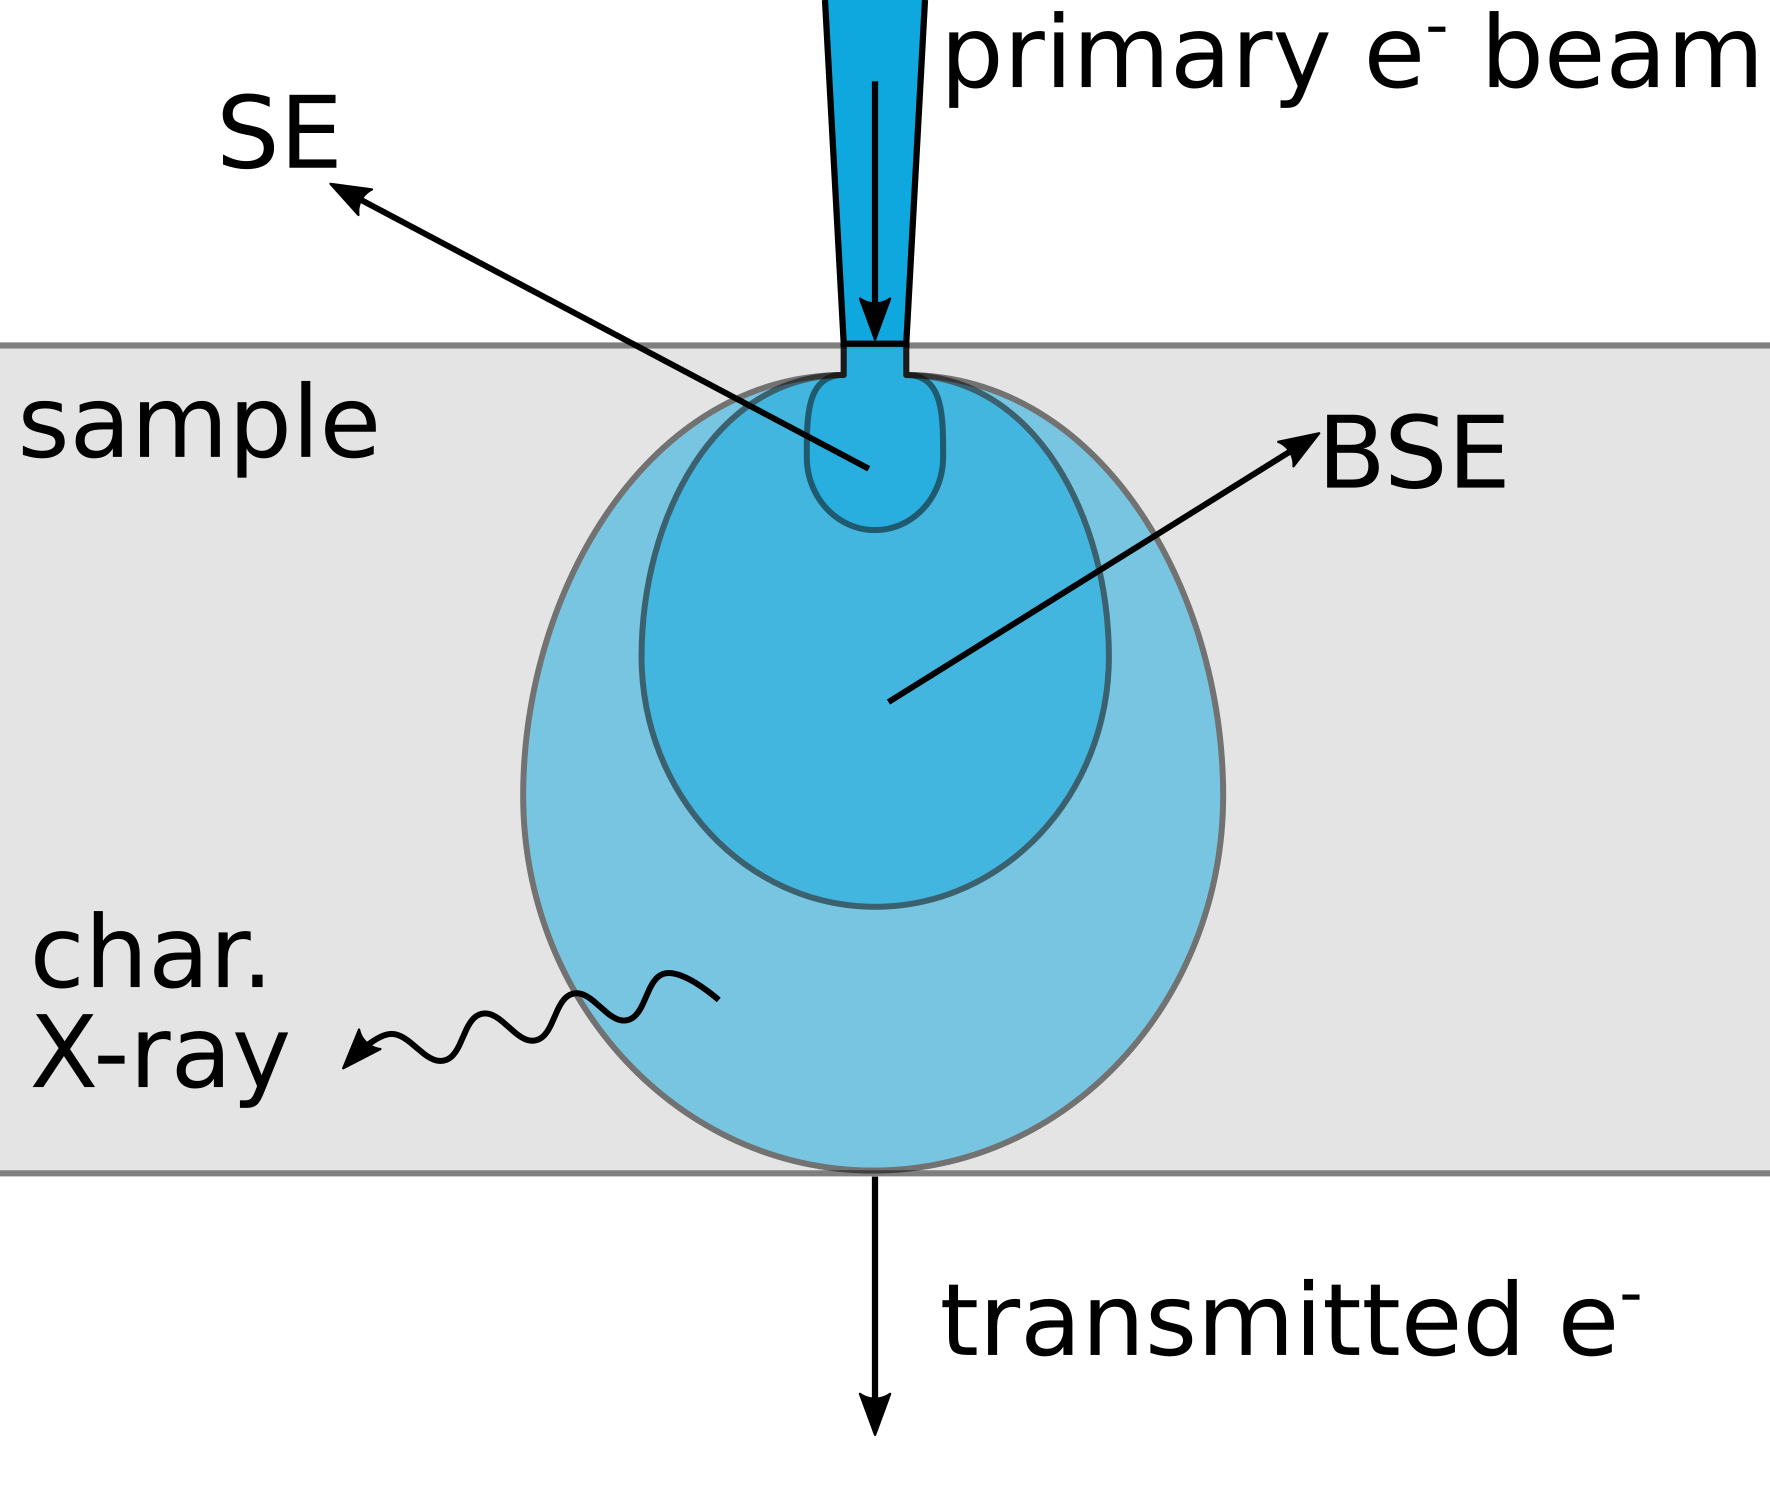
\includegraphics{methods_em_activationVolume}
      \caption{\label{fig:methods:em:activationVolume}Schematic for different phenomena happening upon interaction of an high-energy electron beam with a sample and the typical relative penetration depth of secondary electrons (SE), back-scattered electrons (BSE) and the characteristic X-ray radiation.}
    \end{figure}

    \paragraph{Transmission Electron Microscopy (TEM)}
      measures the transmitted electrons through a thin sample and can achieve a very high resolution below $1 \unit{angstrom}$ (HRTEM).
      In the case of this thesis, TEM is used to obtain a local image of the nanoparticle size and their morphological shape.
      The size distribution of a characteristic dimension of a nanoparticle is evaluated by binning multiple measurements of the dimension in a histogram to obtain the respective number of occurrences for various length scales.
      The number of particles $N$ that need to be measured is typically in the order $N > 100$, such that the histogram is a valid represention of the size distribution.
      The respective measurement error for each bin is estimated as the square root of the counts in that respective bin. \footnote{To understand the estimate of the standard deviation for the height of a bin, the measured particle size can be considered as a random variable with an arbitrary probability density.
      Every bin $i$ for itself can be associated with a probability $p_i$ that the next measurement of X adds to the bin or does not.
      This is essentially a Bernoulli experiment for each bin, where the bin count $n_i$ is a binomial distributed variable.
      The expectation value for the counts in bin $i$ after $N$ total measurements is $\bar{n}_i \eq p_i N$.
      As the bin counts for a large number of measurements represent the probability function, the number of counts become equal to the expectation value for $N \gg 1$ as $p_i \eq n_i / N$ and thus $\bar{n}_i \eq n_i$.
      Furthermore, for a sufficient number of bins, such that $p_i \ll 1$ for every bin, the standard deviation of a binomial distributed variable is given by $\sigma_i \eq \sqrt{N p_i (1-p_i)} \approx \sqrt{n_i}$.}

      To model the size distribution by a simple function, a log-normal distribution function is fit to the histogram
      \begin{align}\label{eq:looselyPackedNP:nanoparticle:lognormalDist}
        p(d; \mu, \sigma) \eq \frac{1}{\sqrt{2\pi} \sigma d} \exp \biggl( - \frac{\log(d) - \log(\mu)}{2 \sigma^2} \biggr),
      \end{align}
      where the parameters $\mu$ and $\sigma$ relate to the expectation value and standard deviation of the size distribution via
      \begin{align}
        \mathrm{E}[d] \eq& \mu e^{\sigma^2/2} \approx \mu,\\
        \mathrm{Std}[d] \eq& \mu e^{\sigma^2/2} \sqrt{e^{\sigma^2} - 1} \approx \mu \sigma,\\
      \end{align}
      with the approximations being only valid for small size distributions $\sigma^2 \ll 1$.

    \paragraph{Scanning Electron Microscopy (SEM)}
      is another EM technique that is used to a large extend in this thesis to study surface and cross-sectional structure of nanostructures deposited on a substrate.
      Here, not the transmitted electrons are detected, but the high-energy back-scattered electrons (BSE) and low-energy secondary electrons (SE) that are produced by the interaction of the electron beam with the sample are of interest.
      Detectors for the different energy scales are set up in the SEM to measure the intensity of these electrons, while the primary electron beam scans pixel by pixel over an area of interest.
      The measured SE are mostly produced at the surface of the sample and therefore give an image of the local topography of the surface, whereas the BSE can be generally generated deeper within the sample and their intensity is more dependent on the relative electron density in the sample.
      In this thesis, the shown micrographs obtained by SEM are always from the BSE detector, as these provided the better contrast in comparison to SE and thereby gave the resolution needed to resolve $10 \unit{nm}$ sized nanoparticles.

    \paragraph{Energy-Dispersive X-ray Spectroscopy (EDX)}
      is a technique to analyze the elemental composition of a sample.
      For this purpose the electron beam is set to a high voltage of typically $\geq 20 \unit{kV}$ and is directed on a sample with a thickness larger than $1 \unit{\textmu m}$.
      The energy of the X-rays emitted from the sample are characteristic for the sample composition and can be measured by a energy-sensitive detector.
      By comparison with literature values for the K$\alpha$, K$\beta$, \ldots energies of the elements, the spectra provide information about which elements are present in the sample and about the relative amount of the elements by the relative intensity of the spectra.
      A caveat is that EDX is typically not reliable in the detection of elements with small atomic numbers below that of \ch{Na}.
\end{document}